\documentclass{amsart}

\usepackage[T1]{fontenc}
\usepackage[utf8]{inputenc}
\usepackage[UKenglish]{babel}
\usepackage{amsmath}
\usepackage{amsthm}
\usepackage{amssymb}
\usepackage{float}
\usepackage{graphicx}
\usepackage{algorithm}
\usepackage{algorithmic}
\usepackage{todonotes}
\usepackage{enumitem}
\usepackage[misc]{ifsym}
\usepackage[foot]{amsaddr}
\usepackage[hidelinks]{hyperref}
\usepackage[style=authoryear,ibidtracker=false,uniquename=false,giveninits=true,terseinits=true,maxbibnames=5,backend=biber]{biblatex}
\renewbibmacro{in:}{}
\addbibresource{lit.bib}

\newcommand{\np}{\mathcal{NP}}
\newcommand{\parent}{\mathrm{parent}}
\newcommand{\mrca}{\mathrm{mrca}}
\newcommand{\rank}{\mathrm{rank}}
\newcommand{\nni}{\mathrm{NNI}}
\newcommand{\rnni}{\mathrm{RNNI}}
\newcommand{\rnniu}{\mathrm{RNNIu}}
\newcommand{\tbr}{\mathrm{TBR}}
\newcommand{\rspr}{\mathrm{rSPR}}
\newcommand{\csort}{\textsc{Caterpillar Sort}}
\newcommand{\findpath}{\textsc{FindPath}}

\newtheorem{definition}{Definition}
\newtheorem{theorem}[definition]{Theorem}
\newtheorem{conjecture}[definition]{Conjecture}
\newtheorem{lemma}[definition]{Lemma}
\newtheorem{corollary}[definition]{Corollary}
\newtheorem{proposition}[definition]{Proposition}

\graphicspath{{figures/}}


\title{The Ranked Nearest Neighbour Interchange space}
\date{\today}
\author{Lena Collienne\textsuperscript{1}}
\email{lena.collienne@postgrad.otago.ac.nz}
\address{\textsuperscript{1}Department of Computer Science, University of Otago, New Zealand}
\author{Mareike Fischer\textsuperscript{2}}
\email{email@mareikefischer.de}
\address{\textsuperscript{2}Institute for Mathematics and Inofrmatics, University of Greifswald, Germany}
\author{Alex Gavryushkin\textsuperscript{1, \Letter}}
\email{alex@biods.org}


\begin{document}

\maketitle

\begin{abstract}

\end{abstract}


% All papers have this section so no need for this heading -- let's wait until a journal pushes us to put it back :)
%\section{Introduction}

%Introduce RNNI as ranked nearest neighbour interchange space, only ultrametric trees considered (extension could be mentioned in the end)

%We use the exact algorithm to calculate all the distances for the examples given in this paper

%Figure of ranked tree in introduction

Although we endeavour to make this paper self-sufficient, we refer the reader to standard textbooks in phylogenetics for terminology \autocite{Felsenstein2004-of, Semple2003-nj, Steel2016-ye}.
Unless is explicit, we follow these textbooks in our terminology.


\section{Definitions}

A \emph{rooted binary phylogenetic tree} on a set $X$ is a pair $(T, \Phi)$ where $T$ is a rooted binary tree with leaf set $\mathcal{L}(T)$ and $\Phi:X \to \mathcal{L}(T)$ a bijective mapping.
\todo{do we need to define leaves and internal nodes, child, parent, subtree, cherry(defined below)?
AG: Only if we use those terms.
Can we use something like a glossary to automatically know what terminology we need to introduce?}
From now on, we assume $X = \{1,\ldots,n\}$ for a fixed number $n \in \mathbb N$ of leaves.

In this paper we study \emph{ranked trees} that are determined by a pair consisting of a rooted binary phylogenetic tree $(T, \Phi)$ on $X = \{1, \ldots, n\}$ for $n \in \mathbb N$, and a rank function.
In the literature ranked trees are often referred to as labelled history in the context of coalescent trees.
The following notion differs from the definition of ranks in that context, since we do not use negative integers as ranks.
A \emph{rank function} on $T$ maps the vertex set of $T$ onto the set $\{0,\ldots,n-1\}$ such that all leaves are assigned rank $0$ and each internal node has rank greater than its children.
The rank of a node $v$ in a ranked tree will be denoted by $\rank(v)$.
For simplicity of notation we use the term \emph{tree} instead instead of ranked tree.

We will identify leaves with their labels and also call them \emph{taxa} (singular: \emph{taxon}) following the systematic biology tradition.
All nodes that are no leafs are called \emph{internal nodes} and edges $(u,v)$ are \emph{internal edge}, if both $u$ and $v$ are internal nodes.
Our definition of ranked tree leads to a natural characterisation of edge lengths within ranked trees:
integer $l$ denotes the \emph{length} of an edge $e=(u,v)$ if $|\rank(v) - \rank(u)| = l$.
Two trees are called \emph{isomorphic} if the underlying rooted phylogenetic trees are isomorphic and the isomorphism preserves ranks of the nodes.

Now we are ready to define the tree space which is the subject of study in this paper, the $\rnni$ graph.
Note that we will define the $\rnni$ graph on ultrametric trees where all leaves have the same rank $0$, and therefore refers to the $\rnniu$ graph as introduced in \autocite{Gavryushkin2017}.
The vertex set of the \emph{$\rnni$ graph} is given by the set of all ranked trees on $n$ taxa.
We introduce two types of operations (\emph{$\rnni$ moves}) connecting trees $T$ and $R$ in this graph by an edge:
A swap of the ranks of two internal nodes ($x$ and $y$) of subsequent ranks ($|\rank(x) - \rank(y)| = 1$) is called a \emph{rank move}.
We say that trees $T$ and $R$ are \emph{connected} by an \emph{$\nni$ move} move if there exist internal edges $e$ in $T$ and $f$ in $R$ both of length one such that the graphs obtained by shrinking $e$ and $f$ to internal nodes are isomorphic.
The above definition follows \autocite{Gavryushkin2017} and is equivalent to the common definition of $\nni$ operations as given in \autocite{Steel2016-ye}.
Trees that are connected by either a rank move or an $\nni$ move are called \emph{$\rnni$ neighbours} or \emph{adjacent in} $\rnni$.
Note that thus defined $\rnni$ graph is a metric space with the standard shortest-path distance.

\begin{figure}[H]
	\centering
	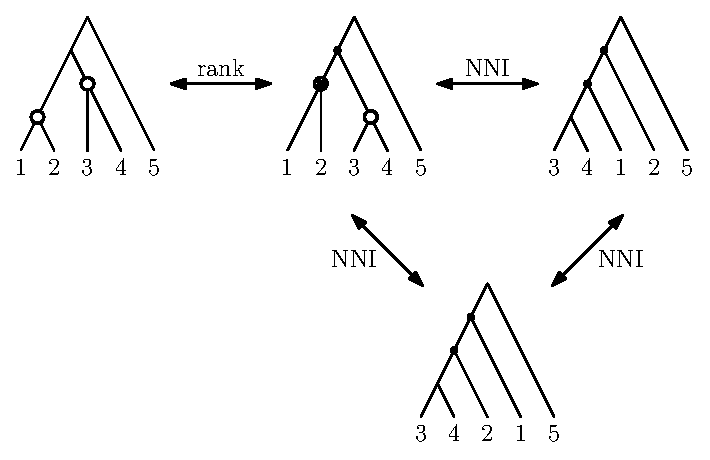
\includegraphics[width=\textwidth]{RNNI}
	\caption{Four trees connected by edges in the $\rnni$ graph. A rank move of $\mrca(\{1,2\})$ and $\mrca(\{3,4\})$ and all $\nni$ moves on the edge highlighted in red are illustrated}
	\label{fig:RNNI}
\end{figure}

\todo{label of taxa in figure shouldn't be numbers}

The following definitions are less standard and required for the results obtained in this paper.
A set $\mathbb S$ of trees is called \emph{convex} if for all pairs of trees $T,R \in \mathbb S$, there exists a shortest path from $T$ to $R$ such that every tree on $p$ is element of $\mathbb S$.

\section{Geometry of $\rnni$}
\label{section:geometry}

This paper is an advance towards the general goal of understanding the geometry of the $\rnni$ space.
In this section we are investigating the geometry by analysing the structure of shortest paths in $\rnni$.
We will start by presenting an algorithm for computing paths in $\rnni$ (Algorithm~\ref{alg:find_path}) that turns out to be an essential tool for our studies.
Using this algorithm, we are able to prove that there is always a shortest path between two caterpillar trees that only consists of caterpillar trees (Theorem~\ref{thm:caterpillar_convex}) in Section~\ref{section:caterpillar_convex}.
In other words, the set of caterpillar trees is convex in $\rnni$.
This distinguishes $\rnni$ from $\nni$ where this does not hold.
One further result, presented in Section~\ref{section:diameter}, directly following from the proof of Theorem~\ref{thm:caterpillar_convex}, is the diameter of $\rnni$.
Finally, we disprove the so-called Split Theorem, conjectured in \autocite{Gavryushkin2017}, and formulate an alternative version of it, the Cluster Theorem (Section~\ref{section:split_theorem}).

We now present an efficient algorithm for computing paths between pairs of trees in $\rnni$.
Throughout this paper we will denote this algorithm by $\findpath$.
We will see that it becomes a central tool for our investigation of shortest paths.

The idea of the algorithm is described in the following.
Each node $v$ of a tree defines a \emph{cluster} $C$, which is the set of taxa descending from the $v$.
We then say that $v$ \emph{induces} the cluster $C$.
Note that the list of all clusters of a tree, if sorted increasingly according to the rank of the corresponding nodes, uniquely defines that tree.
For computing a path from trees $T$ to $R$, we consider clusters $C_1, \ldots, C_{n-1}$ of $R$ where $C_i$ is induced by the node with rank $i$ for $i = 1, \ldots, n-1$.
The so-called \emph{trivial clusters} that are induced by leaves and the root are the same in every tree and do therefore not need to be changed on any path between two trees.
Therefore, the list of clusters $C_1, \ldots, C_{n-1}$, which is ordered increasingly according to the ranks of the corresponding nodes, uniquely defines $R$.
Starting at tree $\hat{T} = T$, $\findpath$ constructs a path where the clusters of $R$ are constructed from bottom to top, using following procedure:
For each $C_i$, find the \emph{most recent common ancestor} $\mrca_{\hat{T}}{C_i}$ (also known as \emph{least common ancestor}) of $C_i$ in current tree $\hat{T}$, that is the internal node with lowest rank that is ancestral to all the taxa in $C_i$.
Update $\hat{T}$ by decreasing the rank of $\mrca_{\hat{T}}{C_i}$ by an $\rnni$ move until it has the same rank $i$ as in $R$. \todo{Do we need to explain why there is always an $\rnni$ move that moves the $\mrca$ down?}
Since we consider the clusters of $R$ such that the ranks of the corresponding internal nodes in $R$ increase, $\mrca_{\hat{T}}{C_i}$ is the parent of cluster $C_i$ in $\hat{T}$ after these $\rnni$ moves.
Thus, repeating this procedure for all clusters of $R$ results in a path between any pair of tress $T, R$, indeed.
Further details, including pseudo-code for $\findpath$, can be found in Section~\ref{section:computation_findpath}.

This algorithm gives an upper bound for the diameter of $\rnni$, which improves the one given in \autocite{Gavryushkin2017}.
Later we will see that this bound is tight.
However, we don't know how good $\findpath$ approximates distances in $\rnni$. \todo{Can we say something about the approximation ratio?}
More details can be found in Section~\ref{section:computation}.

\begin{lemma}
    $\Delta(\rnni) \leq \frac{(n-1)(n-2)}{2}$, where $\Delta(G)$ denotes the diameter of graph $G$.
\end{lemma}

\begin{proof}
    Let us consider the maximum length of a path given by Algorithm~\ref{alg:find_path}.
    In worst case each of the $n-2$ clusters $C$ induced by internal nodes of $R$ with ranks $i = 1, \dots, n-2$, requires $n-1-i$ $\rnni$ moves to move $\mrca(C)$ down in $\hat{T}$.
	Hence, the maximum length of a path computed by that algorithm for any pair of trees is less or equal to $\sum\limits_{i = 1}^{n-2} i = \frac{(n-2)(n-1)}{2}$.
\end{proof}

Lemma~\ref{lemma:distance_delete_taxon} is central for some of the following proofs using induction.

Central for the following inductive proofs is the comparison of the length of a shortest paths $p$ on trees on $n+1$ taxa with a path on $n$ taxa induced by $p$.
The following lemma bounds the length of these induced paths utilising the rank differences of certain internal nodes between start and end tree of $p$.
Henceforth the notion $\parent(x)$ refers to the internal node that is parent of taxon $x$.

\begin{lemma}
    Let $T$ and $R$ be two trees on $n+1$ taxa.
    Let $T{\big|}_n$ and $R{\big|}_n$ be these trees restricted to taxa $1, \ldots, n$, i.e. taxon $n+1$ is deleted from $T$ and $R$ and the thereby arising node of degree two is suppressed.
    Then it is $d(T{\big|}_n, R{\big|}_n) \leq d(T,R) - \delta$ where $\delta:= |\rank_T(\parent(n+1)) - \rank_R(\parent(n+1))|$ is the rank difference of the parent of taxon $x$ between trees $T$ and $R$.
    \label{lemma:distance_delete_taxon}
\end{lemma}

\begin{proof}
    Let $p$ be a shortest path from tree $T$ to $R$ and $p{\big|}_n$ the path resulting from deleting taxon $n+1$ from all trees on $p$.
    This new path $p{\big|}_n$ is then a path from $T$ to $R$.
    Showing that at least $\delta$ $\rnni$ moves are deleted from $p$ to receive $p{\big|}_n$ results in $d(T{\big|}_n,R{\big|}_n) \leq |p{\big|}_n| \leq |p| - \delta = d(T,R) -\delta$ which proves the lemma.
    By the following two observations one can easily see that this claim is true, indeed:
    The rank of an internal node $v$ only changes within an $\rnni$ move if this move is a rank move of $v$ with another node or an $\nni$ move on an edge incident to $v$.
    Furthermore, any $\rnni$ move can change the rank of an internal node by at most one.
    Applying this to $\parent(n+1)$ and knowing that the rank of this node differs by $\delta$ between $T$ and $R$ proves that $d(T{\big|}_n, R{\big|}_n) \leq d(T,R) - \delta$.

    % Alternative: Induction:
    %
    % Induction on $k = d(T,R)$:
    %
    % Basis($k = 1$):
    % If rank of $\parent(n+1)$ changes between $T$ and $R$, it is $d(T{\big|}_n, R{\big|}_n) = 0$ and $|\rank_T(\parent(n+1)) - \rank_R(\parent(n+1))| = 1$ and therefore, $d(T{\big|}_n, R{\big|}_n) = 0 \leq 1 - 1 = d(T,R) - |\rank_T(\parent(n+1)) - \rank_R(\parent(n+1))|$.
    % If on the other hand the rank of $\parent(n+1}$ does not change between $T$ and $R$, it is $d(T{\big|}_n, R{\big|}_n) = d(T,R) = 1$ and $|r_{T}(\parent(n+1}) - r_{R}(\parent(n+1})| = 1$ and therefore, $d(T{\big|}_n, R{\big|}_n) = 1 \leq 1 - 0 = d(T,R) - |r_{T}(\parent(n+1}) - r_{R}(\parent(n+1})|$.
    %
    % Step($k \to k+1$):
    % Let $T$ and $R$ be trees on $n+1$ taxa with distance $d(T,R) = k$.
    % Let $R'$ be the last tree on a shortest path from $T$ to $R$, i.e. $d(T,R') = k$.
    % We can apply the induction hypothesis on $T$ and $R'$ and see that $d(T{\big|}_n, R'{\big|}_n) \leq d(T, R') - |r_{T}(\parent(n+1}) - r_{R'}(\parent(n+1})| := k - m$.
    % Now we differ two cases:
    % \begin{enumerate}
    %     \item $\parent(n+1}$ changes its rank between $R$ and $R'$ or is affected by the $\nni$ move is performed between $R$ and $R'$.
    %
    %     Then the trees $R{\big|}_n$ and $R'{\big|}_n$ are equal. \todo{Is this obivous?}
    %     Therefore, it is $d(T{\big|}_n,R{\big|}_n) = d(T{\big|}_n, R'{\big|}_n) \leq k - m$.
    %     It is either $|r_{T}(\parent(n+1}) - r_{R}(\parent(n+1})| = m+1$, $|r_{T}(\parent(n+1}) - r_{R}(\parent(n+1})| = m$, or $|r_{T}(\parent(n+1}) - r_{R}(\parent(n+1})| = m-1$.
    %     In either case, we have $d(T{\big|}_n,R{\big|}_n) = d(T{\big|}_n, R'{\big|}_n) \leq k - m = (k+1) - (m+1) \leq d(T, R) - |r_{T}(\parent(n+1}) - r_{R}(\parent(n+1})|$.
    %
    %     \item $\parent(n+1}$ has same rank in $R$ and $R'$.
    %
    %     In this case it is $d(T{\big|}_n,R{\big|}_n) \leq d(T{\big|}_n,R'{\big|}_n) + d(R'{\big|}_n, R{\big|}_n) \leq d(T{\big|}_n, R'{\big|}_n) + 1 \leq (k-m)+ 1$.
    %     It also follows that $|r_{T}(\parent(n+1}) - r_{R'}(\parent(n+1})| = |r_{T}(\parent(n+1}) - r_{R}(\parent(n+1})|$ and therefore, we can conclude $d(T{\big|}_n,R{\big|}_n) \leq k-m+1 = k+1-m = d(T,R) -  |r_{T}(\parent(n+1}) - r_{R}(\parent(n+1})|$.
    % \end{enumerate}
\end{proof}

%Following Proposition might not be needed(?)

Related to Lemma~\ref{lemma:distance_delete_taxon} is Proposition~\ref{proposition:lower_bound_distance} which provides a lower bound for the distance of two trees.
Using the same arguments as in the proof of Lemma~\ref{lemma:distance_delete_taxon}, it easily follows that the rank difference of parents of any taxon in two trees gives such a bound.

\begin{proposition}
    Given trees $T$ and $R$ with taxon $x$ that fulfils $|\rank_T(\parent(x)) - \rank_R(\parent(x))| = k$, it follows $d(T,R) \geq k$.
    \label{proposition:lower_bound_distance}
\end{proposition}

\subsection{The set of caterpillar trees}
\label{section:caterpillar_convex}

In this section we restrict our attention to the set of \emph{caterpillar trees} where each internal node has at least one child that is a leaf.
This type of tree is of particular interest in $\rnni$ because shortest paths between such trees in $\rnni$ differ from those in classical $\nni$ space.
This in combination with the importance of caterpillar trees in the proof of $\np$-hardness of $\nni$ distances in \autocite{jiang2000} suggests that understanding the geometry of paths between caterpillar trees helps investigating the complexity of computing $\rnni$ distances.
In particular, we are going to prove that one can always find a shortest path between two caterpillar trees that contains caterpillar trees only, meaning that the set of caterpillar trees is convex in $\rnni$.
We discovered this by computing caterpillar paths using an algorithm to compute shortest paths within the set of caterpillar trees and comparing the results with shortest path in $\rnni$.
This algorithm will be explained in detail later in this section, after demonstrating why finding shortest paths between caterpillar trees builds the basis for understanding the difference between $\nni$ and $\rnni$.
Further details on our computational results can be found in Section~\ref{section:computation}.

Before we start analysing shortest paths between caterpillar trees, we introduce further notations.
A path $p$ between two caterpillar trees $T$ and $R$ that only consists of caterpillar trees is called \emph{caterpillar path}.
If $p$ is shortest among all caterpillar paths between these trees we call it \emph{shortest caterpillar path}, and the length of $p$ will be denoted by $d_c(T,R)$ and is called \emph{caterpillar distance}.

Let us compare shortest paths between caterpillar trees in $\nni$ with those in $\rnni$.
The essential difference is that building a cherry and moving it may give a path that is shorter than a path where the taxa move separately in $\nni$ as it is illustrated out in Figure~\ref{fig:NNI_vs_RNNI}.
There is only one move needed in $\nni$ to build and resolve a cherry, respectively, while the number of moves for moving the cherry is the same as for moving a single taxon.
However, in $\rnni$ space, there are additional rank moves needed for the internal node of the cherry before an $\nni$ move resolves it, because $\nni$ moves are only allowed on edges of length one in $\rnni$.
Therefore, a path where taxa move separately and no second cherry is built, is shortest in $\rnni$.

\begin{figure}[H]
	\centering
	\includegraphics[width=\textwidth]{NNI_vs_RNNI}
	\caption{Paths between caterpillar trees $T$ and $R$: black -- shortest path in classical $\nni$ (ignoring ranks) of length $5$; red -- shortest path in $\rnni$ of length $6$; blue -- path in $\rnni$ which is the natural extension of the shortest path in $\nni$ but has length $8$.}
	\label{fig:NNI_vs_RNNI}
\end{figure}

The above observation already suggests that there is always a caterpillar path that is shortest path between two arbitrary caterpillar trees in $\rnni$.
Indeed, we are going to prove Theorem~\ref{thm:caterpillar_convex} within this section, which states that the set of caterpillar trees is convex in $\rnni$.
Note that this is not true for the $\nni$ space, which is clear from the example in Figure~\ref{fig:NNI_vs_RNNI}.

One can see caterpillar trees as sequences of taxa, ordered non-decreasing according to the ranks of their parents.
$\nni$ moves between caterpillar trees, which are the only possible $\rnni$ moves between those trees, coincide with exchanges of two neighboured elements in the sequence.
In these sequences the first two taxa are somehow equivalent since they build the unique cherry.
$\nni$ moves that change the cherry of a tree refer to exchanges of the first or the second element with the third element of the sequence while exchanges of the first two elements do not change the corresponding tree.
With this observation we can provide an algorithm for computing shortest caterpillar paths by a simple modification of the commonly known \emph{Bubble Sort} algorithm \autocite{knuth1997}.
Throughout this paper this algorithm will be called $\csort$.

Following the observations above, only swaps of the first three elements of a sequence with Bubble Sort need to be adapted for the computation of shortest caterpillar paths.
Let us consider the first three elements $a,b,c$ which appear in this order in a sequence representing a caterpillar tree on a caterpillar path between trees $T$ and $R$.
If the rank of $\parent(c)$ is higher than the ranks of $\parent(a)$ and $\parent(b)$ in $R$, there are no swaps needed for these taxa.
If just one of the two taxa $a$ and $b$ is on the other side of $c$ in $R$, this one swaps position with $c$ in the sequence.
But if both $a$ and $b$ are on the other side of $c$ in $R$, the one that has the parent with highest rank of all these three taxa in $R$ swaps with $c$ at first.
This makes sure that there is no additional swap of $a$ and $b$ needed on the path to $R$.
\todo{Do we need to explain Bubble Sort?}

Lemma~\ref{lemma:caterpillar_dist=diameter} regards caterpillar trees with distance $\frac{(n-1)(n-2)}{2}$ and will be needed for proving the convexity of the set of caterpillar trees in $\rnni$.

\begin{lemma}
    Let $T$ and $R$ be two caterpillar trees.
    $T$ and $R$ have distance $d(T,R) = \frac{(n-1)(n-2)}{2}$ if, and only if, they have caterpillar distance $d_c(T,R) = \frac{(n-1)(n-2)}{2}$.
    \label{lemma:caterpillar_dist=diameter}
\end{lemma}

\begin{proof}
    Let $T$ and $R$ be caterpillar trees.
    Let us first prove that if $d(T,R) = \frac{(n-1)(n-2)}{2}$, it follows $d_c(T,R) = \frac{(n-1)(n-2)}{2}$.
    This easily follows from algorithm $\csort$:
    In each loop $i=1, \ldots, n-2$ of the algorithm there can be at most $n-1-i$ exchanges of taxa.
    It follows that the maximum length of a path computed by this algorithm is $\sum\limits_{k=1}^{n-2} k = \frac{(n-1)(n-2)}{2}$.
    Since there cannot be a caterpillar path shorter than $\frac{(n-1)(n-2)}{2}$ if it is $d(T,R) = \frac{(n-1)(n-2)}{2}$, it follows $d_c(T,R) = \Delta(\rnniu)$.

    For proving the other direction of the statement, let now $T$ and $R$ have caterpillar distance $d_c(T,R) =  \frac{(n-1)(n-2)}{2}$.
    We prove $d(T,R) = \frac{(n-1)(n-2)}{2}$ by induction on the number of taxa $n$ of $T$ and $R$:
    Without loss of generality we can assume that $T$ is the caterpillar tree $(\ldots ((1,2),3), \ldots, n)$.
    Let $R$ be a caterpillar tree with distance $\frac{(n-1)(n-2)}{2}$ to $T$.

    Induction basis: $n=3$\\
    All three trees have distance $1$ from another and are caterpillar trees, hence it is $d(T,R) = d_c(T,R)$ for all trees $T,R$ on $n=3$ taxa.

    Induction step: $n \to n+1$\\
    Induction hypothesis: For trees $T, R$ on $n$ taxa it is $d(T, R) = \frac{n(n-1)}{2}$.\\
    Let $T, R$ be trees on $n+1$ taxa with caterpillar distance $\frac{(n-1)(n-2)}{2}$.
    Therefore, each of the $\frac{(n-1)(n-2)}{2}$ pairs of taxa that is considered when running $\csort$ to compute a path $p$ from $R$ to $T$ exchanges.
    From this we can conclude that taxon $n+1$, whose parent has highest rank in $T$, is part of the cherry of $R$.
    Let us consider the trees $T{\big|}_n$ to $R{\big|}_n$ that result from $T$ and $R$ by deleting taxon $n+1$.
    $\csort$ computes a path from $T{\big|}_n$ to $R{\big|}_n$ that contains the same exchanges of taxa as $p$, except for the $n-1$ first ones on $p$ that involve taxon $n+1$.
    Hence, the caterpillar distance is $d_c(T{\big|}_n, R{\big|}_n) = \frac{n(n-1)}{2} - (n-1)$ = $\frac{(n-1)(n-2)}{2}$.
    So we can apply the induction hypothesis on $T{\big|}_n$ and $R{\big|}_n$ and know that $d(T{\big|}_n,R{\big|}_n) = \frac{(n-1)(n-2)}{2}$.

    According to Lemma~\ref{lemma:distance_delete_taxon}, the distance between $T{\big|}_n$ and $R{\big|}_n$ is at least $d(T{\big|}_n, R{\big|}_n) \leq d(T,R) - |\rank_T(\parent(n+1)) - \rank_R(\parent(n+1))|$.
    We also know $|\rank_T(\parent(n+1)) - \rank_R(\parent(n+1))| = n-1$
    Suppose, contrary to our claim, that there is a path from $T$ to $R$ of length less than $\Delta(\rnniu_{n+1}) = \frac{n(n-1)}{2}$.
    By the above, it follows that $d(T{\big|}_n, R{\big|}_n) \leq d(T,R) - |\rank_T(\parent(n+1)) - \rank_R(\parent(n+1))| < \frac{n(n-1)}{2} - (n-1) < \frac{(n-1)(n-2)}{2}$.
    Since this is a contradiction to $d(T{\big|}_n, R{\big|}_n) = \frac{(n-1)(n-2)}{2}$, it is proven that $d(T,R) = \frac{n(n-1)}{2} $.

\end{proof}

\begin{theorem}
    The set of caterpillar trees is convex.
    \label{thm:caterpillar_convex}
\end{theorem}

\begin{proof}
    We prove the Theorem by backwards induction on the length $l$ of a shortest caterpillar path between two caterpillar trees $T$ and $R$.

    Induction basis: $l = \frac{(n-1)(n-2)}{2}$\\
    With Lemma~\ref{lemma:caterpillar_dist=diameter} one can see that for each pair of caterpillar trees $T$, $R$ with caterpillar distance $d_c(T,R) = \frac{(n-1)(n-2)}{2}$, it is $d(T,R) = d_c(T,R)$, which means that there is a shortest path between $T$ and $R$ that is a caterpillar path.

    Induction step: $l+1 \to l$\\
    Induction hypothesis: For each pair of caterpillar trees with caterpillar distance $l+1$ there is a shortest path between these trees that only consists of caterpillar trees, which means that the distance between these trees is $l+1$.
    Let $T$ and $R$ be caterpillar trees with caterpillar distance $l$.
    We consider the shortest caterpillar path computed by $\csort$.
    Since $l < \frac{(n-1)(n-2)}{2}$, there is one loop $k$ when running $\csort$ where less than $n-2-k$ pairs taxa swap positions.
    It follows that there is a taxon $a$ that has parent with rank $n-2-k$ in $T$ and does not need to move all the way up starting at the cherry in loop $k$.
    Let $b$ be the taxon whose parent has rank one less than the parent of $a$ in the tree at the beginning of loop number $k$.
    We can assume without loss of generality that loop $k$ is the first loop in which the number of swaps is not maximal.
    It follows that $a$ and $b$ must be neighboured taxa in $R$.
    Let us no consider caterpillar tree $R'$ resulting from $R$ by exchanging taxa $a$ and $b$.
    It is clear that $R'$ has caterpillar distance $d_c(T,R') = d_c(T,R) + 1 = l+1$ to $T$ and moreover, $d(R,R') = 1$.
    Hence we can apply the induction hypothesis on $T$ and $R'$ and see that $d(T,R') = l+1$.
    If it were $d(T,R) < l$, we would have $d(T,R') \leq d(T,R) + d(R,R') < l + 1$ which contradicts the induction hypothesis.
    We can conclude $d(T,R) = l$, which completes the proof.
\end{proof}


\subsection{Diameter}
\label{section:diameter}

With the results of Section~\ref{section:caterpillar_convex} we can easily provide the exact diameter of the $\rnni$ graph and hence, improve the bounds for the diameter given in \autocite{Gavryushkin2017}.
Moreover, we can conclude from Lemma~\ref{lemma:caterpillar_diameter} that the maximum distance computed by algorithm $\findpath$, which was dicussed introduced above, equals the diameter of $\rnni$.
This suggests that it gives reasonable estimates of distances.
For further details on the quality of that algorithm we refer the reader to Section~\ref{section:computation}.

\begin{lemma}
	There are two caterpillar trees in $\rnniu$ with distance $\frac{(n-1)(n-2))}{2}$.
	\label{lemma:caterpillar_diameter}
\end{lemma}

\begin{proof}
	Let $T = (( \dots (n,1)2)\dots)n-1)$ and $R = (( \dots (n,n-1)n-2)\dots)1)$.
    According to Theorem~\ref{thm:caterpillar_convex}, there is a shortest path between $T$ and $R$ that is a caterpillar path.
    We can compute a shortest caterpillar path by using $\csort$ as explained above.
    When running this algorithm on $T$ and $R$, taxon $i$ swaps $n-1-i$ times with its right neighbour.
    Therefore, the length of a shortest caterpillar path is $\sum\limits_{i=1}^{n-1}(n-1-i) = \sum\limits_{i=0}^{n-2}i = \frac{(n-1)(n-2)}{2}$.
\end{proof}

\begin{corollary}
    It is $\Delta(\rnniu) = \frac{(n-1)(n-2)}{2}$.
\end{corollary}

%Do we need this?

% \begin{lemma}
% 	Let $T$ and $R$ be two caterpillar trees that both have a leaf labelled by $a$ as part of their cherry.
% 	There is a shortest paths from $T$ to $R$ that is a caterpillar path.
% 	\label{lemma:caterpillar_subset_convex}
% \end{lemma}
%
% \begin{figure}[h]
% 	\centering
% 	\includegraphics[width=0.3\textwidth]{label_internal_nodes}
% 	\caption{The labelling of the caterpillar tree as introduced in the proof of Lemma~\ref{lemma:caterpillar_subset_convex} is unique due to its definition.
% 	}
% 	\label{label_internal_nodes}
% \end{figure}
%
% \begin{proof}
% 	Let $T$ and $R$ be two caterpillar trees, both having a leaf labelled by $a$ as part of their cherry.
% 	Let $p$ be a shortest path from $T$ to $R$.
% 	We introduce a labelling of internal nodes of all trees on $p$ by first defining it for the caterpillar trees $T$ and $R$ and then explaining how the labelling is changed by $\rnni$ moves.
%
% 	In $T$ and $R$ the internal node of the cherry is labelled by the label of its child that is not $a$.
% 	All other internal nodes shall have the same label as their leaf children.
% 	From now on we will identify the leaf labelled by $x$ with $x$ and the internal node labelled by $x$ will be called $int_x$.
% 	An example for a caterpillar tree with internal leaf labels is depicted in Figure~\ref{label_internal_nodes}.
% 	In the following, changes of the internal labelling following $\rnni$ moves are defined:
%
% 	\textbf{Rank moves:}
% 	Within rank moves the labels of internal nodes do not change.
% 	For an example consider Figure~\ref{fig:rank_swap_internal_label}.
%
% 	\begin{figure}[H]
% 		\centering
% 		\includegraphics[width=0.8\textwidth]{rank_swap_internal_label}
% 		\caption{The labelling of the internal nodes that swap ranks (red) do not change within the rank move.
% 		}
% 		\label{fig:rank_swap_internal_label}
% 	\end{figure}
%
% 	\textbf{NNI move:}
% 	Let there be an $\nni$ move on an edge $(int_x, int_y)$ where $\rank(int_x) < \rank(int_y)$ as in Figure~\ref{fig:nni_moves}.
%
% 	\begin{figure}[H]
% 		\centering
% 		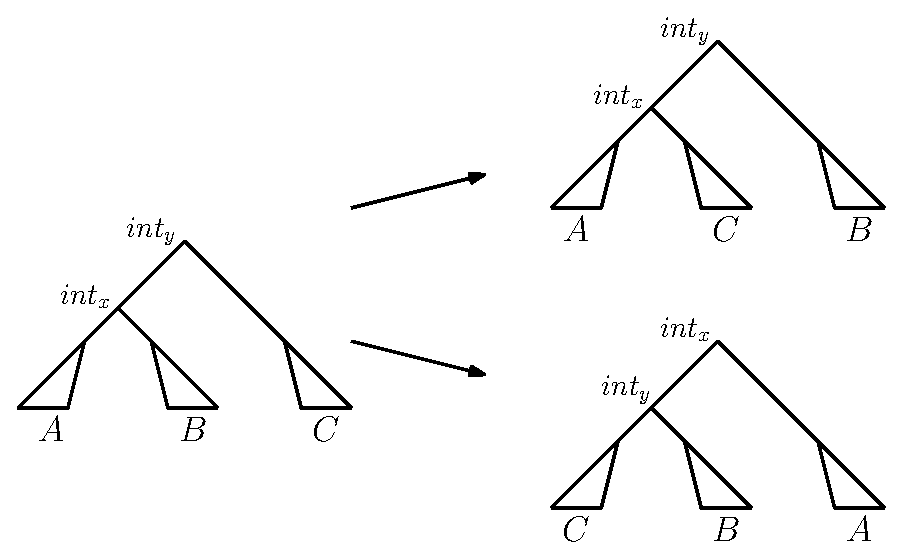
\includegraphics[width=0.7\textwidth]{nni_moves_internal_label}
% 		\caption{Two possible $\nni$ moves on edge $(int_x, int_y)$ where $x \in A, y \in B$.
% 		}
% 		\label{fig:nni_moves}
% 	\end{figure}
%
% 	The nodes incident to the edge after the $\nni$ move are labelled by $int_x$ and $int_y$ as well.
% 	By default, the node that has lower rank than the other one is labelled by $int_x$, the other one by $int_y$.
% 	But if $int_x$ is no ancestor of $x$ or $int_y$ is no ancestor of $y$, we swap the labels of the two new nodes, such that $\rank(int_x) > \rank(int_y)$.
% 	An example of an $\nni$ move and the new labelling is provided in Figure~\ref{fig:nni_example_internal_label}.
%
% 	\begin{figure}[H]
% 		\centering
% 		\includegraphics[width=0.8\textwidth]{nni_example_internal_label}
% 		\caption{The first labelling after the $\nni$ move preserves the ranks of $int_4$ and $int_6$.
% 		But then $int_6$ is not an ancestor of $6$ any more.
% 		Therefore, $int_4$ and $int_6$ have to change their labels.
% 		}
% 		\label{fig:nni_example_internal_label}
% 	\end{figure}
%
% 	We proceed to show that $int_x$ and $int_y$ are ancestors of $x$ and $y$ after an $\nni$ move as described above, respectively.
% 	If $x$ stays in the subtree rooted in the lower node of $e$, this does obviously hold.
% 	We now turn to the case that $x$ is not in the subtree rooted in the lower node of $e$ after the $\nni$ move.
% 	Then the labels of the two internal nodes change such that $\rank(int_x) > \rank(int_y)$.
% 	This makes sure that $int_x$ is an ancestor of $x$.
% 	Thus, it remains to prove that $int_y$ is ancestor of $y$.
% 	In particular, we need to show that $y$ is not in the same subtree $A$ as $x$, whose root has the node labelled by $int_x$ as parent before and after the $\nni$ move.
% 	Let us consider the tree before the $\nni$ move.
% 	$A$ has $|A|$ leaves and $|A| - 1$ internal nodes.
% 	These internal nodes are labelled by some leaves of $A$, because all internal nodes must be labelled by a descendant leaf.
% 	We know that $x \in A$, and the parent of the root of $A$ is labelled by $x$.
% 	All remaining $|A|-1$ leaf labels of $A$ appear as labels of the $|A|-1$ internal nodes of $A$.
% 	From the fact that the internal node labelled by $y$ is not inside $A$ we can conclude that $y$ cannot be a leaf of $A$.
% 	This proves that the labelling of the internal nodes is is well defined and allows a unique identification of internal nodes by their labels.
%
% 	The task is now to prove that there is always a caterpillar path at least as short as the given path $p$.
% 	Therefore, we use the following observation:
% 	Within each $\rnni$ move the ranks of at most two internal nodes change by at most one each.
% 	This is true for both rank moves and $\nni$ moves, according to our definition of the labelling:
% 	Within a rank move two nodes exchange their ranks, while there are not necessarily changes of ranks when $\nni$ moves are performed.
%
% 	On a caterpillar path the only possible moves are $\nni$ moves that change the ranks of two internal nodes by one each.
% 	Therefore, we can construct a caterpillar path $r$ out of $p$:
% 	every time two internal nodes $int_x$ and $int_y$ exchange ranks on $p$, they do so on the caterpillar path $r$ as well.
% 	Since there are moves on $p$ that do not change the ranks of internal nodes, this caterpillar path has length $|r| \leq |p|$.
% 	Hence, there is always a shortest path between $T$ and $R$ that is a caterpillar path.
% \end{proof}

\subsection{Split Theorem}
\label{section:split_theorem}
\todo{Split or Cluster?}

Within this section we will make a further step towards understanding the complexity of computing shortest paths in $\rnni$.
Since the problem of computing distances in the most common tree spaces as $\nni$ \autocite{jiang2000}, $\rspr$ \autocite{Bordewich2005}, or $\tbr$ \autocite{allen2001subtree} is known to be $\np$-hard, it would be desirable to find a tree space that is less complex.
However, it is not known whether computing distances in $\rnni$ is $\np$-hard or not.
The natural approach to solve this question is to compare $\rnni$ and $\nni$ graph to see whether the reason that $\nni$ is $\np$-hard transfers to $\rnni$.
In this section we will consider an important example of shortest paths in $\nni$ that build the key of the proof of its $\np$-hardness.
Afterwards we see that this example cannot transferred to $\rnni$ which is why the so-called Split Theorem, which generalises the example, has been conjectured in \autocite{Gavryushkin2017}.
However, we present a counterexample disproving the Split Theorem (Conjecture~\ref{conjecture:split_theorem}) in its original version and claiming the Cluster Theorem (Conjecture~\ref{conjecture:cluster_theorem}) as alternative version.

The proof of NP-completeness of $\nni$ in \autocite{jiang2000} is based on the fact that following theorem holds in $\nni$.

\begin{theorem}
	There are trees $T,R$ in $\nni$ sharing a cluster which is not shared by any intermediate tree on any shortest path from $T$ to $R$.
	\label{thm:split_nni}
    %The formulation of this lemma is a bit different in Li1996.
    %However, the lemma as stated here follows directly from Li1996.
\end{theorem}

\begin{proof}
	See \autocite{Li1996}.
\end{proof}

In the proof presented in \autocite{Li1996} for Theorem~\ref{thm:split_nni} an example of two trees that share a cluster but have no shortest path that preserves this cluster is given.
The reason that this proof does not work for $\rnni$ is similar to the reason that caterpillar trees are convex in $\rnni$, but not in $\nni$.
Both trees $T$ and $R$ in the example of \autocite{Li1996} have $2n$ taxa and consist of two caterpillar trees that share the root as parent.
The clusters given by the two nodes adjacent to the root are $\{1, \ldots, n\}$ and $\{n+1, \ldots, 2n\}$ in both trees $T$ and $R$.
There is a shortest path in $\nni$ where at first $T$ is transformed to a tree $T'$ with $n$ cherries where each cherry contains one taxon of $\{1, \ldots, n\}$ and one taxon of $\{n+1, \ldots, 2n\}$.
Afterwards, $T'$ is transformed to a tree $R'$ still containing the same cherries as $T'$ but in a way that resolving all these cherries of $R'$ results in $R$.
For proving that this path is shorter than any path preserving the clusters $\{1, \ldots, n\}$ and $\{n+1, \ldots, 2n\}$, the fact that $d_{\nni}(R,R') = d_{\nni}(T{\big|}_{\{1, \ldots, n\}}, R{\big|}_{\{1, \ldots, n\}})$ where $T{\big|}_{\{1, \ldots, n\}}$ and $R{\big|}_{\{1, \ldots, n\}}$ are $T$ and $R$ restricted to taxa $\{1,\ldots,n\}$, respectively, is being used.
However, this does not work in $\rnni$.
Similar to what we observed in the example depicted in Figure~\ref{fig:NNI_vs_RNNI}, there are lots of additional rank moves needed on a similar path in $\rnni$.
Therefore, a path where the two caterpillar trees are sorted separately, is shorter in $\rnni$.
\todo{(1) Do we want this explanation?
(2) If yes, is this explanation sufficient (we never say how we assign ranks to $T$ and $R$)?}



% \todo{Shall we keep this explanation? The problem is that the $\rnni$ path depends on the assignment of ranks to the cherries produced on the path}
% The counterexample presented in \autocite{Li1996} works in $\nni$ because of the following:
% When proving Theorem~\ref{thm:split_nni}, \autocite{Li1996} gives an example of two trees $T$ and $R$ on $2n$ taxa that consist of two caterpillar trees each that share the root as parent.
% The clusters given by the two nodes adjacent to the root are $\{1, \ldots, n\}$ and $\{n+1, \ldots, 2n\}$ in both trees $T$ and $R$.
% Between these there is a shortest path in $\nni$ where at first $T$ is transformed to a tree $T'$ with $n$ cherries where each cherry contains one taxon of $\{1, \ldots, n\}$ and one taxon of $\{n+1, \ldots, 2n\}$.
% Afterwards, $T'$ is transformed to a tree $R'$ still containing the same cherries as $T'$ but in a way that resolving all these cherries of $R'$ results in $R$.
% For proving that this path is shorter than any path preserving the clusters $\{1, \ldots, n\}$ and $\{n+1, \ldots, 2n\}$, the fact that $d_{\nni}(R,R') = d_{\nni}(T{\big|}_{\{1, \ldots, n\}}, R{\big|}_{\{1, \ldots, n\}})$ where $T{\big|}_{\{1, \ldots, n\}}$ and $R{\big|}_{\{1, \ldots, n\}}$ are $T$ and $R$ restricted to taxa $\{1,\ldots,n\}$, respectively, is being used.
% However, this does not work in $\rnni$.
% Introducing new cherries means introducing new internal nodes with new ranks.
% Since there are lots of rank moves needed for an $\rnni$ path similar to the shortest $\nni$ path presented above, the path in $\rnni$ that breaks the clusters $\{1, \ldots, n\}$ and $\{n+1, \ldots, 2n\}$ is no shortest path.

% ^How do we assign the ranks to the new cherry nodes?
% We could either create a path where $R$ and $R'$ have distance equal to $d_{\rnni}(T{\big|}_{\{1, \ldots, n\}}, R{\big|}_{\{n+1, \ldots, 2n\}})$ and have a lot of additional rank moves before and after that part OR
% Build $R$ and $R'$ that contain all the cherries within the least number of moves possible (3n-3) and having a longer path between $R$ and $R'$.
% Also anything in between these two options is possible. Are we able to disprove every option??


Since the example given in \autocite{Li1996} that proves Theorem~\ref{thm:split_nni} in $\nni$ does not work in $\rnni$, a contrary statement was conjectured in \autocite{Gavryushkin2017}.
For understanding this conjecture it is important to realise the connection between edges in a tree and bipartitions of the taxon set of that tree.
By deleting an edge $e$ of a tree $T$ one receives two trees on taxon sets $A$ and $B$ such that $\{A,B\}$ is a partition of the taxon set of $T$.
Note that each edge induces such a bipartition, often written as $A|B$, and that both edges incident to the root of a tree induce the same partition.
As these partitions are commonly referred to as \emph{splits}, the following conjecture was named \emph{Split Theorem} in \autocite{Gavryushkin2017}.

\begin{conjecture}[Split Theorem]
	For the $\rnni$ graph the following statement holds:
	If a partition of leaves given by an edge is present in two trees $T$ and $R$ then the partition is presented in every tree on every shortest path between $T$ and $R$.
	\label{conjecture:split_theorem}
\end{conjecture}


However, we found a simple counterexample to this conjecture:

\begin{figure}[H]
	\centering
	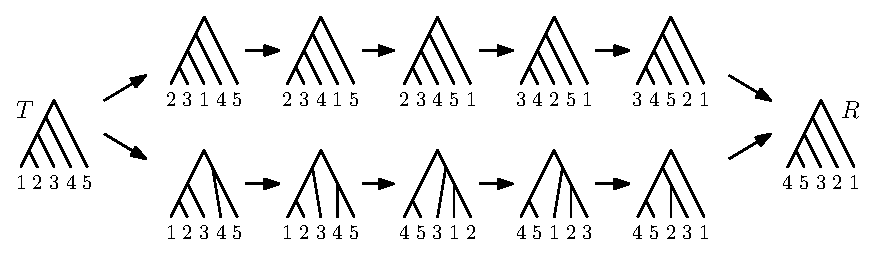
\includegraphics[width=\textwidth]{splitthm_counterexample}
	\caption{The split $123|45$ is present in $T$ and $R$, but the path at the top is a shortest path where none of the trees contains this split.
    However, this split is maintained on the path at the bottom that is a shortest path as well.}
	\label{splitthm_counterexample}
\end{figure}

Since the counterexample in Figure~\ref{splitthm_counterexample} clearly shows that the version of the Split Theorem stated in \autocite{Gavryushkin2017} does not hold, we will now claim an alternative to this conjecture, the \emph{Cluster Theorem}.
Within the Cluster Theorem we are considering clusters instead of splits.
This is motivated by the fact that rooted phylogenetic trees can uniquely be represented by sets of clusters \autocite{Steel2016-ye}, but not by sets of splits as they cannot define the position of the root.
Moreover, a ranked tree can be uniquely determined by ordering the set of clusters increasingly according to the ranks of the internal nodes inducing those clusters.

% \begin{conjecture}[Weak Split Theorem]
% 	For $\rnni$ graph the following statement holds:
% 	if a partition of leaves given by an edge is present in two trees $T$ and $R$ then there exists a shortest path between $T$ and $R$ where this partition is present in every tree on this path.
% 	\label{split_theorem_weak}
% \end{conjecture}
%
% \todo{Do we want to keep the weak version of the split thm? It is stronger than the Cluster Thm!}
%
% The weak Split Theorem (in the version as in Lena's thesis) is computationally proven to hold for trees with up to $6$ taxa ($\sim 38$ min running time on laptop).

\begin{conjecture}[Cluster Theorem]
	For the $\rnni$ graph the following statement holds:
	if two trees $T$ and $R$ contain the same cluster $C$, then $C$ is present as cluster in every tree on every shortest path between $T$ and $R$.
	\label{conjecture:cluster_theorem}
\end{conjecture}

Note that the trees $T, R$ of counterexample~\ref{splitthm_counterexample} share the same set of induced splits, but have distinct sets of clusters.
Furthermore, the example used in $\rnni$ to show that there are trees that share splits that are not present on any shortest path between these trees can be used to prove that the Cluster Theorem does not hold in $\nni$.

\section{Computational results}
\label{section:computation}

In \autocite{Gavryushkin2017} an efficient algorithm for computing the $\rnni$ graph has been introduced.
We implemented this algorithm and could produce the graph for trees with up to $8$ taxa.
This enables us to compute exact distances between trees of this size.
It is in particular possible to compare the exact distances with distances we receive from algorithms we introduced previously and to verify the Cluster Theorem, which was raised in Section~\ref{section:split_theorem}, for small trees.
All algorithms have been implemented with Python and are available online. \todo{link?}

\subsection{Algorithm $\findpath$}
\label{section:computation_findpath}

In Section~\ref{section:geometry} we introduced the algorithm $\findpath$ for computing paths between arbitrary trees in $\rnni$.
Therefore, we can use it as approximation for distances in $\rnni$.
In this section we are providing pseudo-code for $\findpath$ (Algorithm~\ref{alg:find_path}) to provide further insights.
We implemented and tested this algorithm for trees on up to $k$ taxa, for which it gives the exact $\rnni$ distance. \todo{$k = ?$}

\begin{algorithm}[H]
\caption{$\findpath$($T,R$)}
\label{alg:find_path}
\begin{algorithmic}[1]
	\STATE $\hat{T} := T$
	\STATE $p := (T)$
	\FOR {$i = 1, \dots, n-2$}
		\STATE Let $C$ be the cluster induced by node $v$ in $R$ with $\rank(v) = i$
		\WHILE {$\rank(\mrca_{\hat{T}}(C))>i$}
			\STATE Update $\hat{T}$: Decrease $\rank(\mrca_{\hat{T}}(C))$ by an $\rnni$ move \label{alg:line:move_set_down}
			\STATE $p = p+\hat{T}$
		\ENDWHILE
	\ENDFOR
	\RETURN $p$
\end{algorithmic}
\end{algorithm}

Recall that the Section~\ref{section:diameter} revealed that the maximum distance computed by $\findpath$ for an arbitrary pair of trees equals the diameter of $\rnni$.
Thus, if the distance between two trees equals the diameter, $\findpath$ computes the correct distance.
Note that central for proving the convexity of the set of caterpillar trees in Section~\ref{section:caterpillar_convex} was Lemma~\ref{lemma:caterpillar_dist=diameter}.
We therefore aim to find a property for any pair of trees, not only caterpillar trees, with maximum distance $\Delta(\rnni) = \frac{(n-1)(n-2)}{2}$.
Following algorithm $\findpath$, we claim following conjecture:

\begin{conjecture}
    Let $T$ and $R$ be two trees.
    It is $d(T,R) = \frac{(n-1)(n-2)}{2}$ if, and only if, $\findpath(T,R)$ computes a path of this length between $T$ and $R$.
    \label{conjecture:findpath_maxdist_correct}
\end{conjecture}

Provided Conjecture~\ref{conjecture:findpath_maxdist_correct} holds, there is a simple algorithm for computing a tree $R$ with maximum distance from any given tree $T$.
%TODO
%Explain this algorithm, not only Pseudo-Code!

\begin{algorithm}[H]
\caption{MAX\_DISTANCE\_TREE($T$)}
\label{alg:max_dist_tree}
\begin{algorithmic}[1]
	\STATE $R$ only contains cherry taxa $a, b$ of $T$ and has internal node with rank $n-1$
    \STATE In list $L$ all taxa $\{1,\ldots,n\}\setminus\{a,b\}$ are sorted such that the ranks of their parents in $T$ do not decrease
	\FOR {taxon $a$ in $L$}
		\STATE Add an internal node as parent of $a$ on any edge in $R$ such that the new internal node has rank one less than the previously lowest internal node
	\ENDFOR
	\RETURN $R$
\end{algorithmic}
\end{algorithm}

\begin{lemma}
    Let $T$ and $R$ be trees.
    Algorithm~\ref{alg:find_path} ($\findpath$) gives a path of length $\frac{(n-1)(n-2)}{2}$ between $T$ and $R$ if, and only if, $R$ can be generated from $T$ by applying Algorithm~\ref{alg:max_dist_tree}.
    \label{lemma:max_dist_lemmas_equivalence}
\end{lemma}

According to Lemma~\ref{lemma:max_dist_lemmas_equivalence}, Conjecture~\ref{conjecture:findpath_maxdist_correct} is equivalence to the conjecture that two trees have maximum distance if, and only if, one can be obtained from the other by applying Algorithm~\ref{alg:max_dist_tree}.

%TODO
%proof (short explanation)

If Conjecture~\ref{conjecture:findpath_maxdist_correct} is correct, it directly would follow that the radius of $\rnni$ is $rad(\rnni) = \Delta(\rnni) = \frac{(n-1)(n-2)}{2}$, where $rad(G) = \min\limits_u \max\limits_v d(u,v)$ for graph $G$ and nodes $u$ and $v$ in $G$.

\subsection{Connecting Computations and Proofs}
\todo{How shall we structure this?}

In Section~\ref{section:caterpillar_convex} we already indicated that computing distances between trees in $\rnni$ by using the algorithms introduced in previous sections has been important for understanding shortest paths.
Moreover, these algorithm, in particular $\findpath$ and $\csort$, also became a substantial part of some of the in Section~\ref{section:geometry}.

We can also substantiate the Cluster Theorem, which remains to be a conjecture, by proving it computationally for up to $k$ taxa. \todo{k=?, do we provide implementation?}
Together with the analytical results of the previous section, this strongly supports our claim that the Cluster Theorem is true.

%Max Distance Trees Algorithm (+ connection to MRCA algorithm)

\section{Ideas}
\todo{Which ideas do we want to keep? Shall this become an 'open problems/future work' section?}

Following are some ideas that did not lead to major results so far:
% idea for description of max distance caterpillar trees:

\begin{lemma}
    Let $T$ and $R$ be caterpillar trees.
    It is $d_c(T,R) = \Delta(\rnni)$ if, and only if, $T$ and $R$ share no induced triplet.
    \todo{define induced triplets}
\end{lemma}

This Lemma does only hold for caterpillar trees and not for trees with more than one cherry.
Furthermore, triplets do not represent ranked trees uniquely as they do not contain information about the ranks of internal nodes (but they can uniquely define caterpillar trees as these only have one cherry)

\begin{proof}
    % Insert the proof here
    Fix $T = (\ldots(1,2) \ldots ,n)$, use induction on $n$ and $\csort$ (taxon $n$ must be in cherry of $R$ if distance is max).
\end{proof}

If this conjecture is true, we have that $\Delta(\rnni) = rad(\rnni)$.

According to Algorithm~\ref{alg:max_dist_tree}, the number of trees with maximum distance to a given tree $T$ depends on the number of cherries of $T$ and the ranks of their internal nodes.
For caterpillar trees it is $(n-1)!$.
The number of caterpillar trees with distance $\Delta(\rnni)$ from a given caterpillar tree is $2^{n-2}$.



%If this is true, we can follow that radius = diameter


\subsection{Partition lattice}

% Define Partition Lattice $\Pi_n$ and max chains in that lattice!

\begin{theorem}
	The $\rnni$ space on $n$ taxa is isomorphic to the space of maximum chains of the partition lattice $\Pi_n$ where two maximum chains are connected by an edge if, and only if, they differ by exactly one partition.
\end{theorem}


\printbibliography

\end{document}
